\documentclass[border=4pt]{standalone}

\usepackage{amsmath}
\usepackage{tikz}
\usepackage{mathdots}
\usepackage{yhmath}
\usepackage{cancel}
\usepackage{color}
\usepackage{siunitx}
\usepackage{array}
\usepackage{multirow}
\usepackage{amssymb}
\usepackage{gensymb}
\usepackage{tabularx}
\usepackage{booktabs}
\usetikzlibrary{fadings}
\usetikzlibrary{patterns}
\usepackage{pgfplots,amsmath}

\begin{document}

 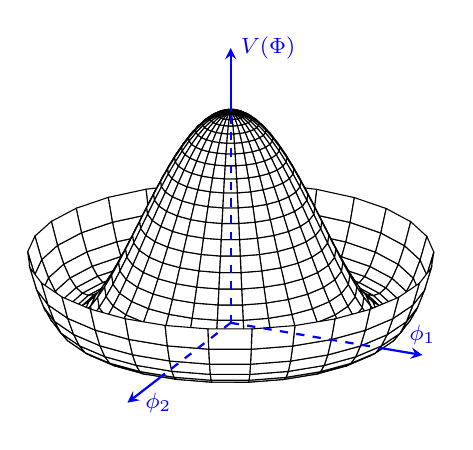
\begin{tikzpicture}
        \begin{axis}[
            hide axis,
            %axis lines=middle,
%            axis on top,
%            axis line style={blue,dashed,thick},
%            ymin=-2,ymax=2,
%            xmin=-2,xmax=2,
%            zmin=-2,zmax=2,
            samples=30,
            domain=0:360,
            y domain=0:1.25,clip=false
        ]
        \addplot3 [surf, shader=flat, draw=black, fill=white, z buffer=sort]
           ({sin(x)*y}, {cos(x)*y}, {(y^2-1)^2});
        \draw[blue,thick,dashed] (axis cs:0,0,0) -- (axis cs:1,0,0)
                    node[below,font=\footnotesize]{$$};
        \draw[blue,thick,-stealth] (axis cs:1,0,0) -- (axis cs:1.3,0,0)
                    node[above,font=\footnotesize]{$\phi_1$};
        \draw[blue,thick,dashed] (axis cs:0,0,0) -- (axis cs:0,-1,0)
                    node[left=2mm,font=\footnotesize]{$$};
        \draw[blue,thick,-stealth] (axis cs:0,-1,0) -- (axis cs:0,-1.5,0)
                    node[right=1mm,font=\footnotesize]{$\phi_2$};
        \draw[blue,thick,dashed] (axis cs:0,0,0) -- (axis cs:0,0,1)
                    node[left=2mm,font=\footnotesize]{$$};
        \draw[blue,thick,-stealth] (axis cs:0,0,1) -- (axis cs:0,0,1.3)
                    node[right,font=\footnotesize]{$V ( \Phi ) $};
        \end{axis}
    \end{tikzpicture}

\end{document}
